\documentclass[a4paper,12pt]{article} 
\usepackage{geometry}
\geometry{
	a4paper,
	total={170mm,257mm},
	left=20mm,
	top=20mm,
}
\usepackage{titlesec}
\titlelabel{\thetitle.\quad} %точка в section

%%% Работа с русским языком
\usepackage{cmap}                           % поиск в PDF
\usepackage{mathtext} 			 	       % русские буквы в формулах
\usepackage[T2A]{fontenc}               % кодировка
\usepackage[utf8]{inputenc}              % кодировка исходного текста
\usepackage[english,russian]{babel}  % локализация и переносы

%Математика
\usepackage{amsmath,amsfonts,amssymb,amsthm,mathtools} % AMS
\usepackage{icomma} % "Умная" запятая

%% Шрифты
\usepackage{euscript}	 % Шрифт Евклид
\usepackage{mathrsfs} % Красивый матшрифт

%% Команды
\DeclareMathOperator{\const}{\mathop{const}}

%% Перенос знаков в формулах
\newcommand*{\hm}[1]{#1\nobreak\discretionary{}
	{\hbox{$\mathsurround=0pt #1$}}{}}

%%% Заголовок
\author{Шерхалов Денис Б02-204}
\title{Лабораторная работа 2.1.6 \\
	\textbf{Эффект Джоуля-Томсона}}
\date{\today}

\begin{document}
	
	{\Large \maketitle}

	\paragraph*{Цель работы:} 1) Определение изменения температуры углекислого газа при протекании через малопроницаемую перегородку при разных начальных значениях давления и температуры; 2) вычисление по результатам опытов коэффициентов Ван-дер-Ваальса <<a>> и <<b>>.
	
	\paragraph*{В работе используются:} трубка с пористой перегородкой; труба Дьюара; термостат; термометры; дифференциальная термопара; микровольтметр; балластный баллон; манометр.
	
	\section{Введение}
	Эффектом Джоуля–Томсона называется изменение температуры газа, медленно протекающего из области высокого в область низкого давления в условиях хорошей тепловой изоляции. В разреженных газах, которые приближаются по своим свойствам к идеальному газу, при таком течении температура газа не меняется. Эффект Джоуля–Томсона демонстрирует отличие исследуемого газа от идеального.
	
	В работе исследуется изменение температуры углекислого газа при медленном его течении по трубке с пористой перегородкой. Трубка 1 хорошо теплоизолирована. Газ из области повышенного давления $P_1$ проходит через множество узких и длинных каналов пористой перегородки 2 в область с атмосферным давлением $P_2$. Перепад давления  $\Delta P = P_1 - P_2$ из-за большого сопротивления каналов может быть заметным даже при малой скорости течения газа в трубке. Величина эффекта Джоуля–Томсона определяется по разности температуры газа до и после перегородки.
	
	Рассмотрим стационарный поток газа между произвольными сечениями I и II трубки (до перегородки и после нее). Пусть, для определенности, через трубку прошел 1 моль углекислого газа; $\mu$ — его молярная масса. Молярные объемы газа, его давления и отнесенные к молю внутренние энергии газа в сечениях I и II обозначим соответственно $V_1$, $P_1$, $U_1$ и $V_2$ , $P_2$ , $U_2$. Для того чтобы ввести в трубку объем $V_1$, над газом нужно совершить работу $A_1$ = $P_1 V_1$. Проходя через сечение II, газ сам совершает работу $A_2$ = $P_2$ $V_2$. Так как через боковые стенки не происходит ни обмена теплом, ни передачи механической энергии, то
	\begin{equation}
		A_1-A_2 = \left(U_2+\frac{\mu v_2^2}{2}\right)-\left(U_1+\frac{\mu v_1^2}{2}\right).
	\end{equation}
	В уравнении (1) учтено изменение как внутренней (первые члены в скобках), так и кинетической (вторые члены в скобках) энергии газа. Подставляя в (1) написанные выражения для $A_1$ и $A_2$ и перегруппировывая члены, найдем
	\begin{equation}
		H_1-H_2 = \left(U + P_1 V_1 \right) - \left(U_2 + P_2 V_2 \right) = \frac{1}{2}\mu\left(v_2^2-v_1^2\right)
	\end{equation}
	
	Сделаем несколько замечаний. Прежде всего отметим, что в процессе Джоуля–Томсона газ испытывает в пористой перегородке существенное трение, приводящее к ее нагреву. Потери энергии на нагрев трубки в начале процесса могут быть очень существенными и сильно искажают ход явления. После того как температура трубки установится и газ станет уносить с собой все выделенное им в пробке тепло, формула (1) становится точной, если, конечно, теплоизоляция трубки достаточно хороша и не происходит утечек тепла наружу через ее стенки.
	
	Второе замечание связано с правой частью (2). Процесс Джоуля–Томсона в чистом виде осуществляется лишь в том случае, если правой частью можно пренебречь, т. е. если макроскопическая скорость газа с обеих сторон трубки достаточно мала. У нас сейчас нет критерия, который позволил бы установить, когда это можно сделать. Поэтому мы отложим на некоторое время обсуждение вопроса о правой части (2), а пока будем считать, что энтальпия газа не меняется.
	
	Рассмотрим выражение:
	\begin{equation}
		\mu_{\text{Д-Т}} = \frac{\Delta T}{\Delta P} \approx \cfrac{\cfrac{2a}{RT}-b}{C_p}
	\end{equation}
	
	Из формулы (3) видно, что эффект Джоуля–Томсона для не очень плотного газа зависит от соотношения величин $a$ и $b$, которые оказывают противоположное влияние на знак эффекта. Если силы взаимодействия между молекулами велики, так что превалирует «поправка на давление», то основную роль играет член, содержащий $a$, и
	\[ \frac{\Delta T}{\Delta P} > 0, \]
	то есть газ при расширении охлаждается ($\Delta t < 0$ так как всегда
	$\Delta P < 0$). В обратном случае (малые a):
	\[ \frac{\Delta T}{\Delta P} < 0, \]
	то есть газ нагревается ($\Delta t < 0$ так как по-прежнему $\Delta P < 0$).
	
	Этот результат нетрудно понять из энергетических соображений. Как мы уже знаем, у идеального газа эффект Джоуля–Томсона отсутствует. Идеальный газ отличается от реального тем, что в нем можно пренебречь потенциальной энергией взаимодействия молекул. Наличие этой энергии приводит к охлаждению или нагреванию реальных газов при расширении. При больших $a$ велика энергия притяжения молекул. Это означает, что потенциальная энергия молекул при их сближении уменьшается, а при удалении — при расширении газа -- возрастает. Возрастание потенциальной энергии молекул происходит за счет их кинетической энергии -- температура газа при расширении падает. Аналогичные рассуждения позволяют понять, почему расширяющийся газ нагревается при больших значениях $b$.
	
	Как следует из формул, при температуре $T_i$ коэффициент $\mu_\text{д-т}$ обращается в нуль. Используя связь между коэффициентами $a$ и $b$ и критической температурой, найдем:
	\begin{equation}
		T_{инв}=\frac{2a}{bR}, \qquad
		T_{инв}=\frac{27}{4}T_{кр}
	\end{equation}
	
	При температуре $T_\text{инв}$ эффект Джоуля–Томсона меняет знак: ниже температуры инверсии эффект положителен ($\mu_\text{д-т} > 0$, газ охлаждается), выше $T_\text{инв}$ эффект отрицателен ($\mu_\text{д-т} < 0$, газ нагревается).	
	
	
	\begin{figure}[h!]
		\centering{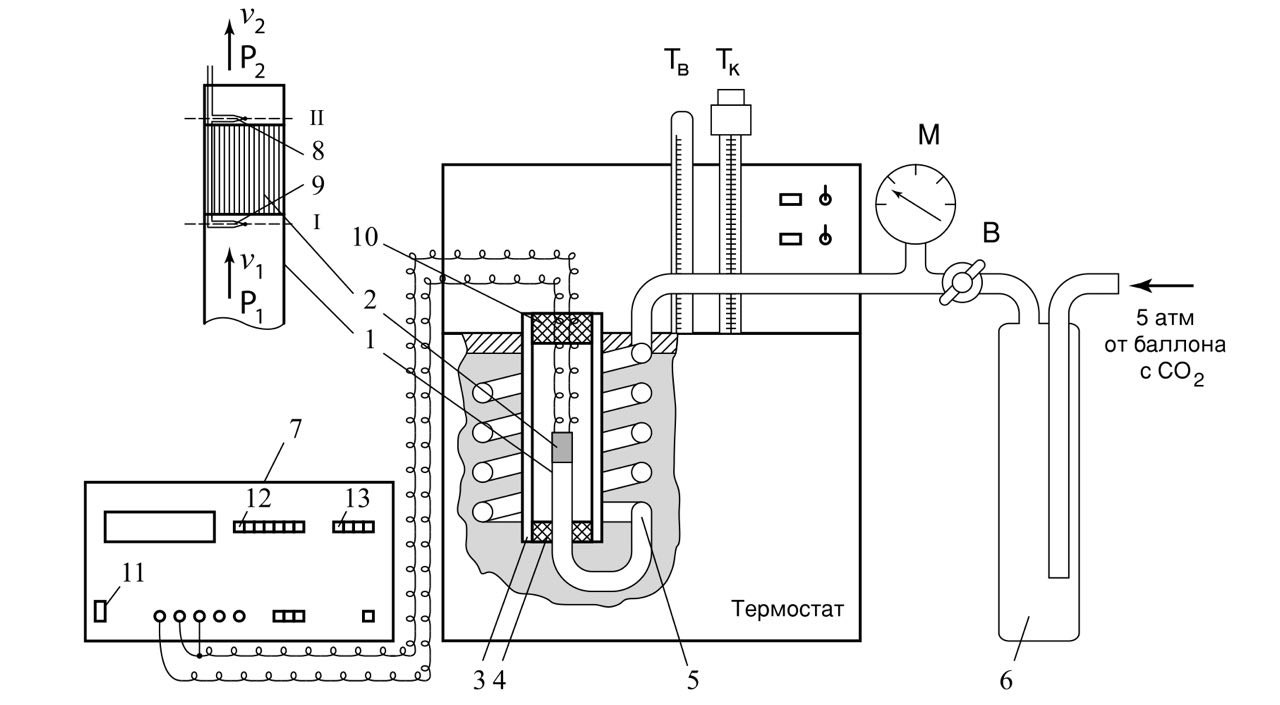
\includegraphics[width=0.75\textwidth]{pic1.jpg}}
		\caption[]{\label{fig:1} Схема установки для изучения эффекта Джоуля–Томсона}
	\end{figure}
	

	\section{Выполнение}
	\begin{enumerate}
		\item Убедившись в том, что термостат залит водой, а все электрические приборы заземлены. Установим на контактном термометре температуру  регулирования, близкую к комнатной $T_1 = T_к = 20.80^\circ C$.
		
		\item Включим вольметр и иземерим паразитные ЭДС при $\Delta P = 0$, получим $U_0 = 1 \, мкВ$. Откроем регулирующий вентиль В настолько, чтобы избыточное давление составило $\Delta P = 4 \, бар$. Теперь будем постепенно понижая давление, выжидать установления равновесия и снимать показания вольтметра. Провести соответствующие измерения удалось 4 раза.
		Далее $\Delta U = 1 \, мкВ$
		
		
		\item В результате построения Графиков №1-4 соответственно по Таблицам №1-4 имеем такие соотношения (Таблица №5):
		
		\begin{table}[h!] 
			\caption{Измерение при $T_1 = 20.80^\circ C$,$\;$ $\alpha\frac{мкВ}{^\circ C} = 40.3$,$\;$ $\delta T = 0.02^\circ C$}
			\begin{center}
				\begin{tabular}{|*{6}{l|}} \hline
					$\Delta P$, бар & 4.0 & 3.5 & 3.0 & 2.5 & 2.0 \\ \hline
					$U - U_0$, мкВ & -118 & -97 & -75 & -56 & -37 \\ \hline
					$\Delta Т$, $^\circ C$ & -2.93 & -2.41 & -1.86 & -1.39 & -0.92 \\ \hline
				\end{tabular}
			\end{center}
		\end{table}

		\begin{table}[h!] 
			\caption{Измерение при $T_2 = 30.00^\circ C$,$\;$ $\alpha\frac{мкВ}{^\circ C} = 41.15$,$\;$ $\delta T = 0.02^\circ C$}
			\begin{center}
				\begin{tabular}{|*{6}{l|}} \hline
					$\Delta P$, бар & 4.0 & 3.5 & 3.0 & 2.5 & 2.0 \\ \hline
					$U - U_0$, мкВ & -111 & -90 & -65 & -48 & -34 \\ \hline
					$\Delta Т$, $^\circ C$ & -2.70 & -2.19 & -1.58 & -1.17 & -0.83 \\ \hline
				\end{tabular}
			\end{center}
		\end{table}
	
		\begin{table}[h!] 
			\caption{Измерение при $T_3 = 40.00^\circ C$,$\;$ $\alpha\frac{мкВ}{^\circ C} = 42.05$,$\;$ $\delta T = 0.02^\circ C$}
			\begin{center}
				\begin{tabular}{|*{6}{l|}} \hline
					$\Delta P$, бар & 4.0 & 3.5 & 3.0 & 2.5 & 2.0 \\ \hline
					$U - U_0$, мкВ & -103 & -84 & -65 & -43 & -30 \\ \hline
					$\Delta Т$, $^\circ C$ & -2.45 & -2.00 & -1.55 & -1.02 & -0.71 \\ \hline
				\end{tabular}
			\end{center}
		\end{table}
	
		\begin{table}[h!] 
			\caption{Измерение при $T_4 = 50.00^\circ C$,$\;$ $\alpha\frac{мкВ}{^\circ C} = 42.9$,$\;$ $\delta T = 0.02^\circ C$}
			\begin{center}
				\begin{tabular}{|*{6}{l|}} \hline
					$\Delta P$, бар & 4.4 & 4.0 & 3.5 & 3.0 & 2.5 \\ \hline
					$U - U_0$, мкВ & -106 & -94 & -76 & -60 & -41 \\ \hline
					$\Delta Т$, $^\circ C$ & -2.47 & -2.19 & -1.77 & -1.40 & -0.96 \\ \hline
				\end{tabular}
			\end{center}
		\end{table}

		\begin{table}[h!] 
			\caption{Коэффициенты наклона графиков $\Delta T (\Delta P)$ при различных температурах}
			\begin{center}
				\begin{tabular}{|*{6}{l|}} \hline
					Номер & $Т, ^\circ C$ & $\mu,\; \frac{K}{бар}$ & $\mu_{min},\; \frac{K}{бар}$ & $\mu_{max},\; \frac{K}{бар}$ & $\Delta \mu,\; \frac{K}{бар}$ \\ \hline
					1 & 20.80 & -1.01 & -0.96 & -1.06 & 0.05 \\ \hline
					2 & 30.00 & -0.95& -0.89 & -0.98 & 0.05 \\ \hline
					3 & 40.00 & -0.89 & -0.83 & -0.91 & 0.04 \\ \hline
					4 & 50.00 & -0.80 & -0.76 & -0.84 & 0.04 \\ \hline
				\end{tabular}
			\end{center}
		\end{table}
		
	
		\item Теперь по Таблице №5 построим Графиков №5 $\mu(T^{-1})$.
		$$k = -670 \frac{K^2}{бар},\quad k_{min} = -976 \frac{K^2}{бар},\quad k_{max} = -390 \frac{K^2}{бар},\quad \Delta k = 293 \frac{K^2}{бар},\quad \varepsilon_{k} \approx 43.7\%$$
		
		$$c = 1.26 \frac{K}{бар},\quad c_{min} = 0.37 \frac{K}{бар},\quad c_{max} = 2.26 \frac{K}{бар},\quad \Delta c = 0.95 \frac{K}{бар},\quad \varepsilon_{c} \approx 74.7\%$$
		
		Далее воспользуемся формулой (3):
		
		$$k = \dfrac{2a}{c_pR} \; \Rightarrow \; a = \dfrac{k \, c_pR}{2} = (1.11\pm0.48) \frac{Па\cdot м^6}{моль^2}$$
		
		$$с = \dfrac{b}{c_p} \; \Rightarrow \; b = c \, c_p = (5.04\pm3.76)\cdot10^{-4} \frac{м^3}{моль}$$
		
		Используя формулу (4), по полученным параметрам газа Ван-дер-Ваальса вычислим: 
		$$T_{инв} = \dfrac{2a}{bR} = 530 \, К, \quad \Delta T_{инв} = \dfrac{2}{R}\left(\dfrac{\Delta a \, b + \Delta b \, a}{b^2}\right) = 625 \, К, \quad \varepsilon_{T_{инв}} \approx 117.9\%$$

\end{enumerate}

\newpage 

\section{Вывод}
	Полученные нами в результате эксперимента значения для $a$ и $b$ получились довольно сильно отличающимися от теоретических значений $a^*$ и $b^*$ для углекислого газа.
	$$a = (1.11\pm0.48) \, \frac{Па\cdot м^6}{моль^2}, \quad \varepsilon_{a} \approx 43.7\%, \quad a^* = 0.36 \, \frac{Па\cdot м^6}{моль^2}$$
	$$b = (5.04\pm3.76)\cdot10^{-4} \, \frac{м^3}{моль}, \quad \varepsilon_{b} \approx 74.7\%, \quad b^* = 0.42\cdot 10^{-4} \, \frac{м^3}{моль}$$
	
	Полученное из значений $a$ и $b$ значение $T_{инв}$ получилось так же сильно отличающимся от теоретического $T_{инв}^*$:
	$$T_{инв} = (530\pm625) \, К, \quad \varepsilon_{T_{инв}} \approx 117.9\%, \quad T_{инв}^* = 2053 \, К$$
	
	Проведя этот эксперимент, мы удостоверились в неприменимости модели Ван-дер-Ваальса в данной лабораторной работе. Полученные зависимости оказались линейны, как и предсказывала теория, но характеризующие коэффициенты этих зависимостей разительно отличаются от теоретических предсказаний. \\
	
			
	\begin{figure}[h!]
		\centering{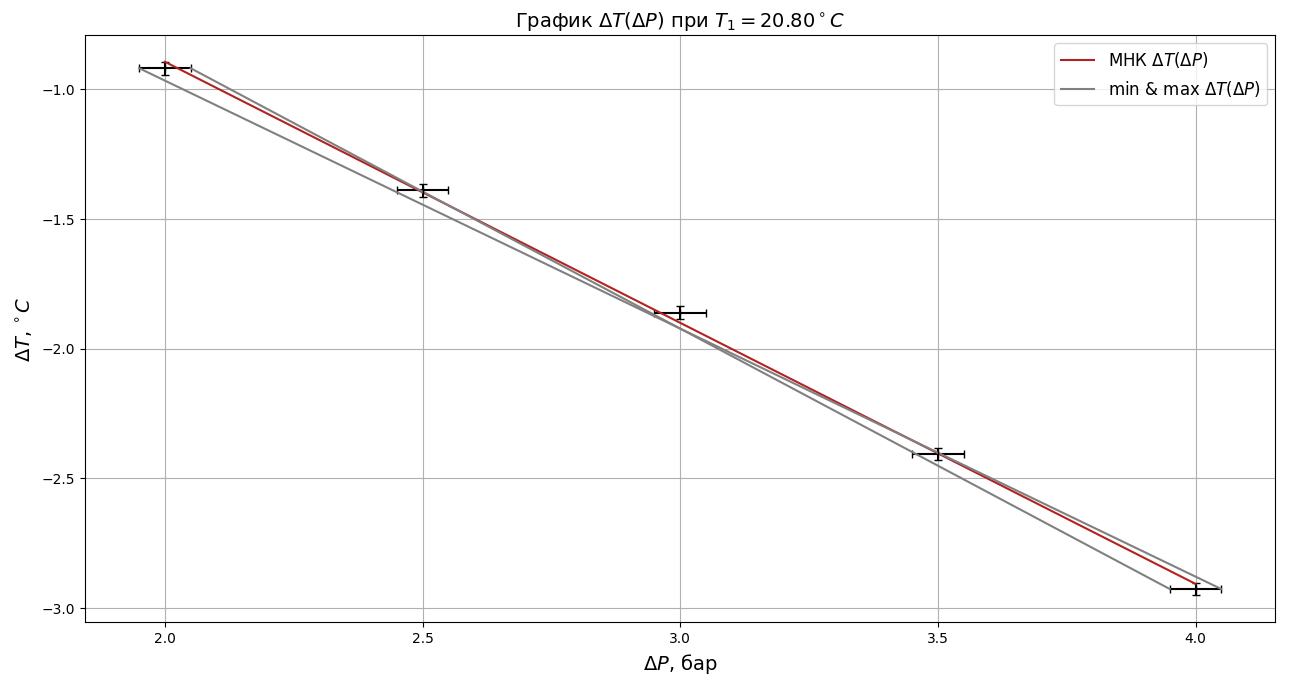
\includegraphics[width=1.00\textwidth]{t20.png}}
		\caption[]{\label{fig:2} График №1}
	\end{figure}

	\begin{figure}[h!]
		\centering{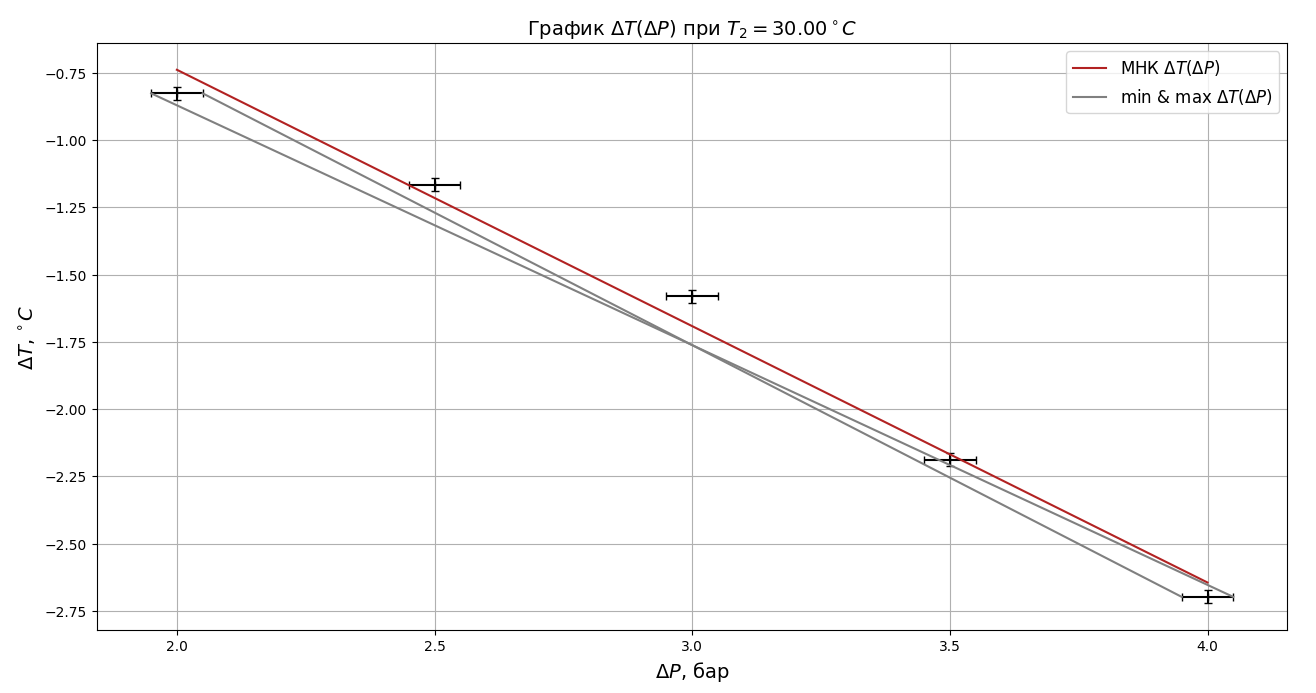
\includegraphics[width=1.00\textwidth]{t30.png}}
		\caption[]{\label{fig:3} График №2}
	\end{figure}

	\begin{figure}[h!]
		\centering{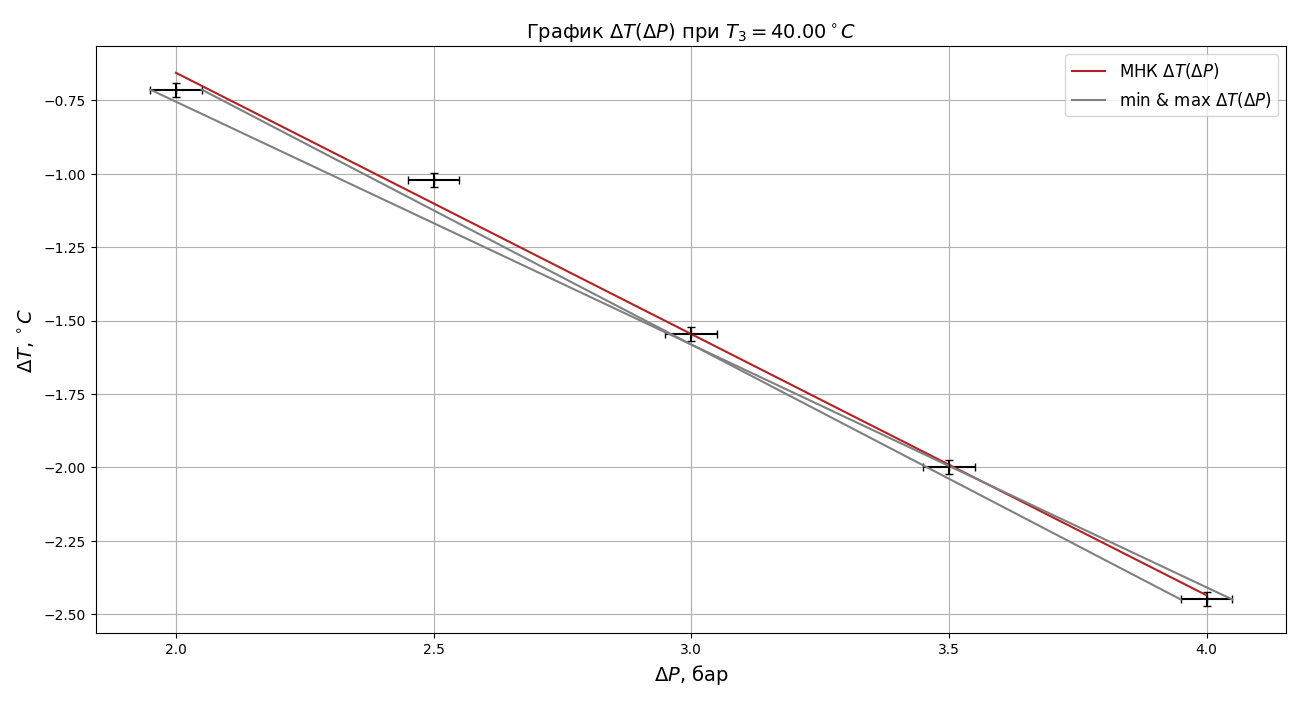
\includegraphics[width=1.00\textwidth]{t40.png}}
		\caption[]{\label{fig:4} График №3}
	\end{figure}

	\begin{figure}[h!]
		\centering{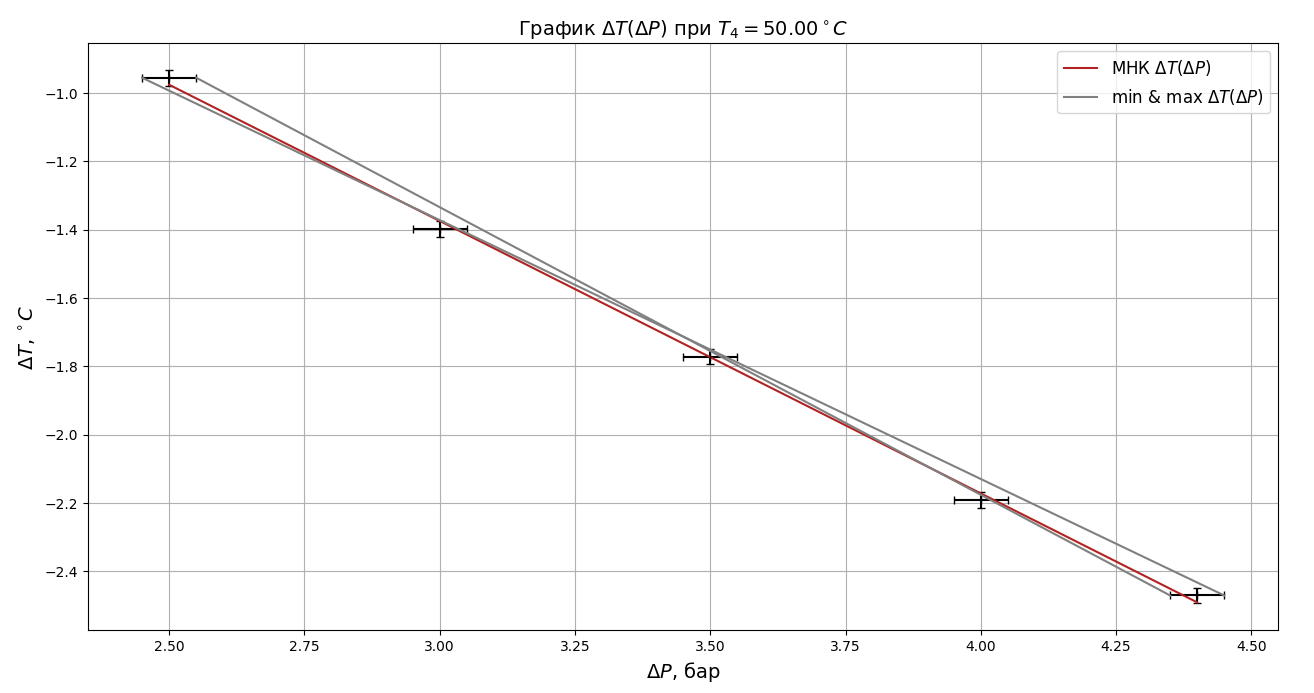
\includegraphics[width=1.00\textwidth]{t50.png}}
		\caption[]{\label{fig:5} График №4}
	\end{figure}

	\begin{figure}[h!]
		\centering{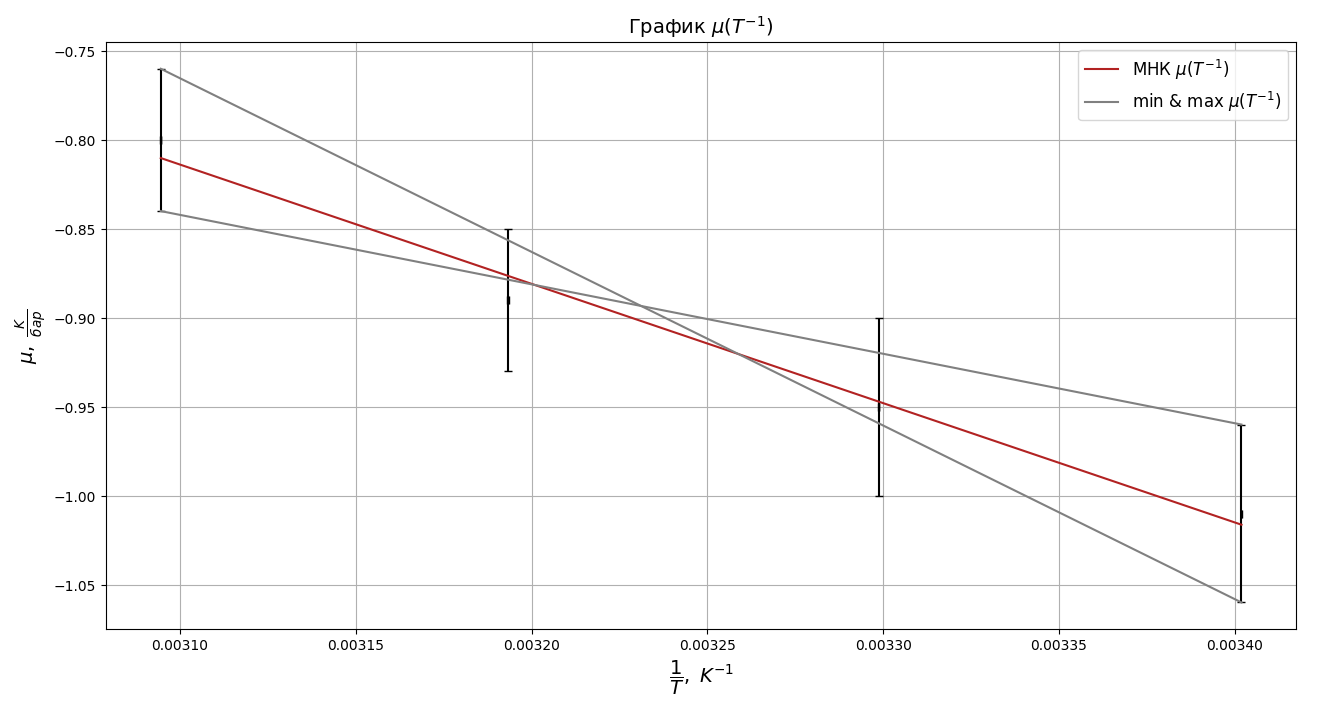
\includegraphics[width=1.00\textwidth]{gr5.png}}
		\caption[]{\label{fig:6} График №5}
	\end{figure}

\end{document}